
\documentclass{article}
\usepackage{graphicx}				
\usepackage{mathtools}	
\usepackage{hyperref}
\usepackage{caption}

\begin{document}
\title{Exam assignment: Implementing Akima spline}
\author{Jedrzej Jawor}
\date{19/06/2018}
\maketitle

\section{Introduction}
This report seeks to implement the Akima sub spline and an another cubic sub-spline and compare them with the cubic spline.
\\
This is a combination of the "Akima spline" and "Yet another cubic sub-spline" exercises from the available exam exercises.
I chose to do both, as "Akima spline" (which I originally did) turned out not to be a part of the valid exam exercises.

\section{Theory}
Interpolation is a process where one constructs a smooth function to fit a set of discrete data points.
This is often done in order to approximate experimental values at points where no data is available.
\\
A spline, S(x), is a piecewise polynomial used for interpolation between two points in a discrete data set:
\begin{equation}
\label{eq:spline}
S(x)=S_i(x), x \in [x_i,x_{i+1}],
\end{equation}
for i=[1,n-1] being the index of the tabulated points.
$S_i$ is a polynomial of order k.
\\
Splines for a discrete data set are calculated by demanding the continuity of the splines and their 
derivatives at the tabulated points \cite{Prakprog}.
\\
The efficiency of splines as interpolating functions varies as splines are
prone to wiggling.
\\
One of the more common choices is a cubic spline (k=3). Cubic splines (cplines) usually have high precision 
but they can also be prone to wiggling if the interpolated set has a large discontinuity or outliers.
\\
\\
If higher precision near such point is desired, a sub-spline can be used. Sub splines are variations
 on the spline method that modify a boundary condition of the spline in order to achieve some form of improvement.
\\
One such sub spline is the Akima sub-spline (aspline).
Asplines are especially useful for data sets with discontinuities as they wiggle much less 
than csplies. However, they come with drawbacks, sacrificing maximal differentiability by 
treating one of the coefficient as a free variable used for wiggle reduction instead of demanding continuity of 
the second derivative.
\\
The method and equations for calculating coefficients for csplines and asplines, on which the code used in this 
*project is based on, come from \cite{Prakprog}.

\subsection{Cubic sub-spline}
The other spline that will be used in this project is a cubic sub-spline (cs-spline). This spline requires 
that we know the derivatives of the tabulated function. So we need a data set:
\begin{equation}
\label{eq:cs1}
x_i,y_i,p_i | i=1...n.
\end{equation}
Where $p_i$ is the derivative at the i'th point.
\\
The i'th cs-spline has the same form as a cubic spline:
\begin{equation}
\label{eq:cs2}
S_i(x)=a_i+b_i h + c_i h^2 +d_i h^3.
\end{equation}
Where $h=(x-x_i)$.
In order to find the proper coefficients ($a_i, b_i, c_i, d_i$) for the spline, we require that four boundary conditions be 
satisfied.
\begin{enumerate}
\item $S_i(x_i)=y_i \Rightarrow a_i=y_i$
\item $S'(x_i) = p_i \Rightarrow b_i=p_i$
\item $S(x_{i+1}) = y_{i+1} \Rightarrow c_i = \frac{dy_i-b_i dx_i -d_i dx_i^3}{dx_i^2}$
\item $S'(x_{i+1} = p_{i+1} \Rightarrow d_i = \left(\frac{dp_i}{3 dx_i^2}-\frac{1}{3 dx_i^3}(dy_i-b_i dx_i)
\right) \left(1+\frac{1}{3}\right)^{-1}$
\end{enumerate}
Here I used: $dx_i=x_{i+1}-x_i$, $dy_i=y_{i+1}-y_i$ and $dp_i=p_{i+1}-p{i}$, $S'$ is the derivative of 
$S$ with respect to x.
\\
The four conditions are sufficient for finding all coefficients as 
$c_i$ can be found after finding $d_i$. It is therefore possible to find all 
cs-splines using only the tabulated function and its derivative.
 
\section{Results and Discussion}
Using the equations for asplies and csplines from \cite{Prakprog}, an aspline for a 
manually tabulated data set with two large outliers is constructed. The derivatives at each point 
are evaluated using a quadratic spline and used for constructing a cs-spline. A cspline is also constructed 
and plotted so that the sub-splines may be compared to it.
\\ 
The discrete points and the splines are shown in figure \ref{fig:man}.
It can be seen that the akima spline wiggles much less that the cubic spline. The cs-spline on the other 
hand seems to wiggle much more. I think this is a result of the quadratic spline giving a poor estimate of 
the derivative.
\\
In order to check if the derivative is the reason for the poor quality of the cs-spline, I make another data 
set where the derivatives are manually tabulated together with the x,y points. Again, aspline, cspline and 
cs-spline are constructed, see figure \ref{fig:man2a}.
\\
The manual estimate of the derivative makes the cs-spline wiggle much less. It wiggles less than the cspline.
\\
The Akima spline is clearly the superior option if one is in need of a spline for a data set with outliers. 
The cs-spline on the other hand seems only to be useful if one has a precise estimate of the derivatives at 
the tabulated points.
\clearpage
\begin{figure}[h]
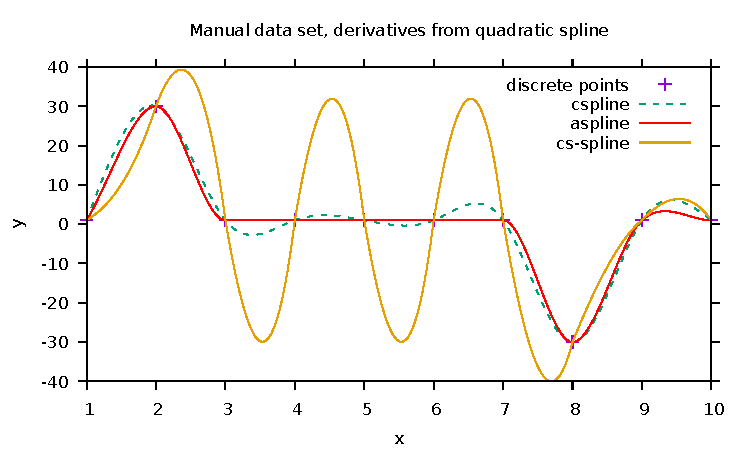
\includegraphics[width=\linewidth]{manualaspline2.pdf}
\caption{Aspline and cs-spline for a manually tabulated data set with derivatives found using a quadratic spline.}
\label{fig:man}

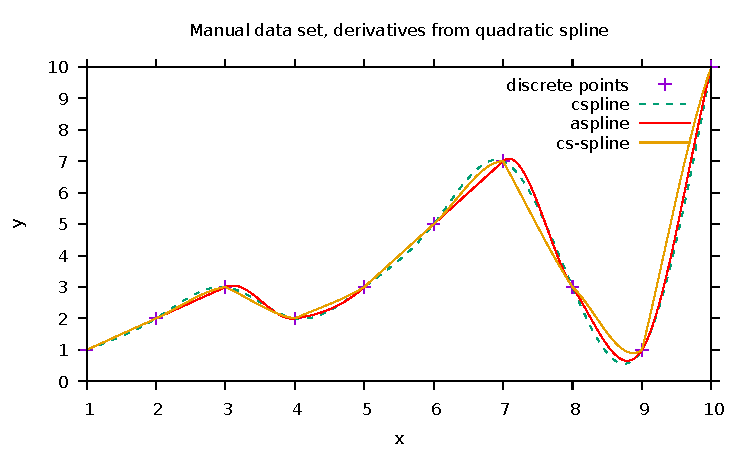
\includegraphics[width=\linewidth]{manualaspline.pdf}
\caption{Aspline and cs-splne for a manually tabulated data set with manually tabulated derivatives.}
\label{fig:man2a}
\end{figure} 
\clearpage

I also want to test the derivatives and integrals of the aspline and cs-spline.
For this purpose a sine function $$f(x) = sin(x)$$ is tabulated in discrete steps. The derivative is tabulated
using the analytic expression $\frac{d}{dx}f(x)=cos(x)$.
The sine was chosen as I can compare the derivatives and integrals with the analytic solutions. 
\\
The a- and cs-splines for $f(x)$ are constructed and their 
derivative and the second derivative are found by differentiation. The splines are plotted in figure 
\ref{fig:sin} while the plots of the 
derivatives are shown in figures \ref{fig:d} and \ref{fig:d2}.
The analytic derivatives are also plotted.
\\
The first derivative seems to be quite bad for both the aspline and cs-spline. They both follow the general 
trend but seem to behave oddly close to the tabulated points.
The second derivatives are even worse. The aspline and cs-spline both become discontinuous.
\\
In both cases, it seems that the cspline is a better option than the two subsplines if one is interested in finding the 
derivatives of the tabulated points.
\begin{figure}
\centering
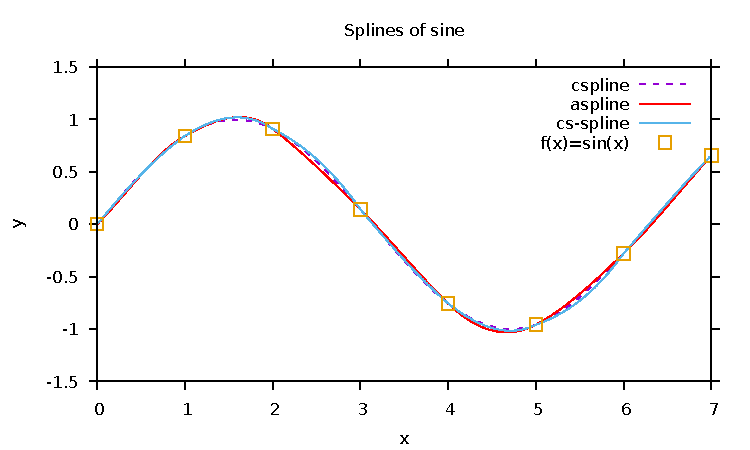
\includegraphics[width=\linewidth]{sinsplines.pdf}
\caption{Aspline and cs-spline for $f(x)$.}%
\label{fig:sin}
\end{figure}

\begin{figure}
\centering
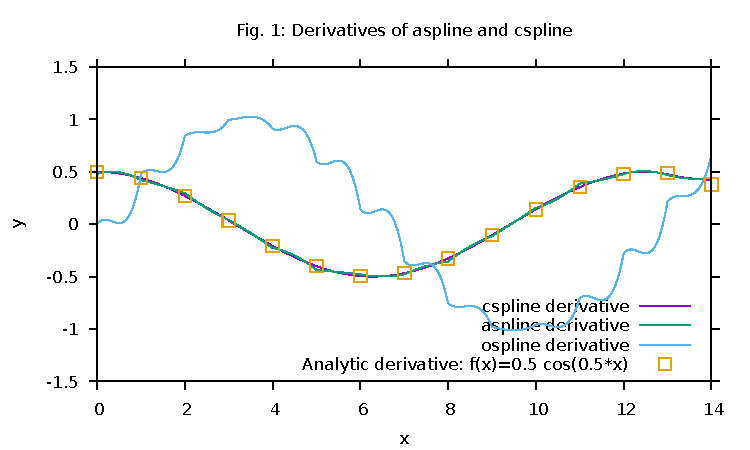
\includegraphics[width=\linewidth]{dsplines.pdf}
\caption{Derivative of aspline and cs-spline for $f(x)$.}%
\label{fig:d}

\centering
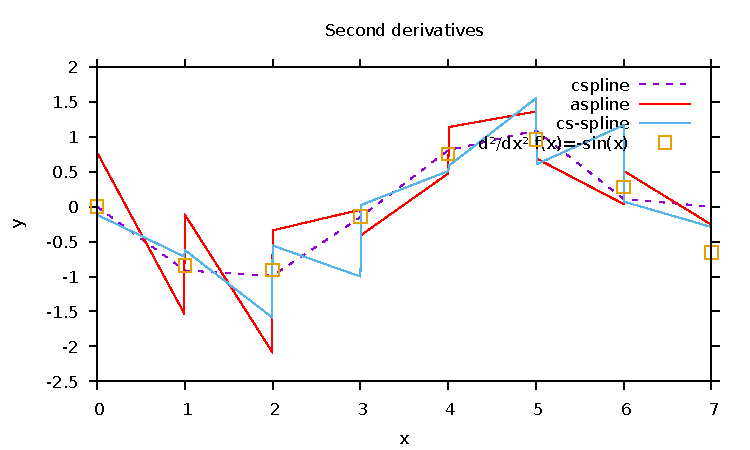
\includegraphics[width=\linewidth]{d2splines.pdf}
\caption{Second derivative of cspline and cs-spline for $f(x)$.}%
\label{fig:d2}
\end{figure} 
\clearpage
Now the integration of the aspline and cs-spline is tested. Again using the sine function $f(x)$.
The analytical integral of $f(x)$ from 0 to 4 is found to be:
\begin{equation}
\int_0^4 f(x) = 1.65364. 
\end{equation}

The aspline integration yields:
\begin{equation}
\int_0^4 aspline = 1.6510. 
\end{equation}

The cspline integration  yields:
\begin{equation}
\int_0^4 cspline = 1.65076. 
\end{equation}

The cs-spline integration  yields:
\begin{equation}
\int_0^4 \text{cs-spline} = 1.68317. 
\end{equation}

So the integration seems to work quite well for both the cs-spline and aspline (at least for a nice analytic function like sine).
The cs-splines seems to be the worst one, but the error is quite small at 0.02.
\clearpage
\begin{thebibliography}{99}
\bibitem{Prakprog}
  Practical programming course book on interpolation.\\
  \emph{PrakProg: Interpolation.pdf},\\
 \url{http://86.52.112.181/~fedorov/numeric/book/interpolation.pdf}\\

\end{thebibliography}

\end{document}
